\section{The Trip Itinerary Planning Problem}
\label{sec:problem}

We now introduce the \emph{Trip Itinerary Planning (TRIP) Problem}.
We assume a city with different points of interest (POIs),
represented as a graph where each POI is a node.  Every pair of POIs
is connected by multiple edges that represent the mode of transport
from one POI to the other.  Thus, if there are two modes of
transport---walking and taxi---there will be two edges between every
pair of POIs.  The weights on an edge $e$ is a tuple $\langle t_e,
c_e \rangle$ that represent the time of travel and the cost of travel
respectively for the particular travel mode.  The time of travel is
typically measured using a constant speed.  Thus, the distance
between the pair of POIs is divided by the constant speed to convert
to time.  Similarly, the taxi cost is computed using a fixed formula
on the distance.  For walking, the cost is $0$.  Each POI $v$ has a
tuple $\langle t_v, c_v, U_v \rangle$ associated with it that
represents the time it takes to visit the POI, the cost (entry fees,
etc.) and the utility a traveler gets by visiting the POI
respectively.  We get this information from \ab{how??}.  While the
time to visit may change from one traveler to another, in this work,
we keep this fixed.  We do, however, let the time of visit of a POI
vary (\ab{Sec.~\ref{dynamic}}) for a user, with the associated
utility also changing.  Additionally, a POI may have a feasible
time-interval of visit in a day (say, a sunset spot, which can be
visited only in the afternoon from 4-6 pm), beyond which visiting it
gives an utility of $0$.  Each POI is also marked with a category or type (e.g.,
park, museum, etc.).  Finally, we have a total time budget and a cost
budget.  Both the time and the cost budgets are spent in traveling as
well as visiting the POIs.  The objective of the \emph{TRIP} problem
is to \emph{find an itinerary}, i.e., a sequence of POIs, that
\emph{maximizes the total utlity} of visiting the POIs under the
given time and cost budget.  The itinerary is prepended by a source
point (e.g., a hotel or an airport) and appended by a destination
point (again, hotel, airport, etc.).  The time and cost to travel
from the source to the first POI and the from the last POI to the
destination has to be also taken into account.

An itinerary $I$ of $n$ POIs is, thus, represented as a sequence
%
\begin{align}
	I = [ S, v_1, \dots, v_n, D ]
\end{align}
%
The total time spent for itinerary $I$ is
%
\begin{align}
	t(I) = t_{S,v_1} + t_{v_1} + t_{v_1,v_2} + t_{v_2} + \dots + t_{v_{n-1,v_n}} + t_{v_n} + t_{v_n,D}
\end{align}
%
which takes into account both the travel time and visiting time.  Similarly,
the total cost of itinerary $I$ is 
%
\begin{align}
	c(I) = c_{S,v_1} + c_{v_1} + c_{v_1,v_2} + c_{v_2} + \dots + c_{v_{n-1,v_n}} + c_{v_n} + c_{v_n,D}
\end{align}
%
which again takes into account both the travel time and visiting time.  The
utility obtained from $I$ is
%
\begin{align}
	U(I) = U_{v_1} + U_{v_2} + \dots + U_{v_n}
\end{align}
%
Given a time budget $T$ and a cost budget $C$, the TRIP problem is to find the
itinerary $I$ that maximizes $U(I)$ subject to the budget constraints:
%
\begin{align}
	& \arg\max_I U(I) \\
	\text{subject to } & t(I) \leq T \text{ and } c(I) \leq C
\end{align}

The traveler may put additional constraints on the itinerary such as
a particular POI must be visited (e.g., Eiffel Tower in Paris).  She
may also put restrictions in the form that not more than $k$ POIs of
the same category may be included and/or at least one POI of a particular
category must be included, etc.  She may also put in ordering
constraints, such as a temple must be visited before a museum, etc.  The feasible itinerary $I$ must satisfy all these
constraints.

\ignore{

ordering constraint: si + ... <= M (big-M constraint)

}

\ignore{

In this work, we introduce the \emph{Trip Itinerary Planning (TRIP) Problem},
which is formulated as follows. The city is represented as a multimodal graph
of points of interest (POIs), with every pair of POIs connected by two edges
corresponding to walking and taxi travel. The taxi speed is $s_t$ and walking
speed is $s_w$. Using these, the time to travel from one POI to another is
calculated. Similarly, there is a cost per distance unit $c_t$ for taxi (the
corresponding cost for walking is $c_w = 0$), using which the cost of traveling
from one POI to another is computed. Every POI has a \emph{utility score},
which is its relative attractiveness or significance to the tourist. Given a
cost and a time budget, the basic problem is to \emph{find an itinerary}, i.e.,
a sequence of POIs, that \emph{maximizes the overall utility} obtained from the
chosen POIs. The core of the system is formulated as a Mixed-Integer Linear
Programming (MILP) problem, solved using the Gurobi Optimizer\footnote{\ab{cite
the tool}}, a powerful tool for mathematical optimization.
%The goal of the MILP model is to maximize the total utility obtained from the
%chosen POIs in the resulting itinerary, subject to a rich set of real-world
%constraints.

The itinerary is a linear, day-wise sequence of POIs that the tourist traverses
in the city over multiple days, while adhering to daily time constraints and
overall cost constraint. Let $V$ denote the set of POIs in the city. Each POI
has its associated opening and closing time, i.e., the time window in which it
can be explored by the tourists. Also, each POI has a weekly schedule and
specific operating days on which it can be visited.

\ab{This section is too much to-and-fro; there is not much of a flow -- we need to discuss}

Each POI \( v_i \in V \) has the following features:

\begin{itemize}
    \item \( U(v_i) \): Utility Score associated with each POI
    \item \( ot(v_i) \): Opening time of POI
    \item \( ct(v_i) \): Closing time of POI
    \item \( t(v_i) \): Average visit time spent by tourists on the POI
    \item \( c(v_i) \): Entrance fee for the POI.
\end{itemize}

\noindent \textbf{Multimodal Graph Representation:}
This problem is modeled using a multimodal graph \( G = (V, E) \) where:

\begin{itemize}
    \item \( V = \{v_1, ..., v_N\} \) denotes the set of all Points of interest of the city
    \item \( E \) contains two distinct edges between every pair of POIs \( (v_i, v_j) \), corresponding the two modes of travel:
    \begin{itemize}
        \item \textbf{Walking Edge} \( e^{w}_{i,j} \) is characterized by:
        \begin{itemize}
            \item \( t^{w}_{i,j} \): Time required to walk from \( v_i \) to \( v_j \).
            \item \( c^{w}_{i,j} \): Cost associated with walking (usually zero).
        \end{itemize}
        \item \textbf{Taxi Edge} \( e^{t}_{i,j} \) is characterized by:
        \begin{itemize}
            \item \( t^{t}_{i,j} \): Time required to travel by taxi.
            \item \( c^{t}_{i,j} \): Cost of travel by taxi.
        \end{itemize}
    \end{itemize}
    \item \textit{days} is the set of all days.
\end{itemize}

\noindent \textbf{Objective Function}\\
To create multi-day itinerary, the optimization ensures a balanced distribution across all days. The objective is to \textbf{maximize the total utility score across all days}.

The decision variable \( y_{i,d} \in \{0,1\} \) indicates whether POI \( v_i \) is selected on day \( d \). The objective function is:
\begin{align}
U(I) &= \sum_{d \in \text{days}} \sum_{i = 1}^{N} U(v_i) \cdot y_{i,d} \label{eq:multi_day_binary}
\end{align}

This equation computes the total utility $U(I)$ of the multi-day itinerary by summing the utilities of all selected POIs across all days.

The basic constraints of the system are described below:

\begin{itemize}

\item \textbf{Time Budget Constraint}\\
This constraint ensures that the total time taken i.e. the sum of visit and travel times is under the user specified time budget for each day.

\begin{align}
\label{mul_day_9}
    & \sum_{i \ne j} t^{w}_{i,j} \cdot w_{i,j,d}
    + \sum_{i \ne j} t^{t}_{i,j} \cdot x_{i,j,d}
    + \sum_{i \in V} t(v_i) \cdot y_{i,d} \leq H
\end{align}

where H is the time budget specified by user. The user can specify different time budgets for the first day, last day, and intermediate days to account for flight or train arrival and departure timings.
\\[1ex]
\item \textbf{Cost Budget Constraint} \\
 This constraint ensures that the total cost of the trip, including both taxi travel and POI entry fees, remains within the cost budget specified by the user.

\begin{align}
\label{mul_day_25}
\sum_{d \in \text{days}} \sum_{(i,j) \in I} \left(c^{w}_{i,j} \cdot w_{i,j} + c^{t}_{i,j} \cdot x_{i,j} \right) + \sum_{d \in \text{days}} \sum_{i \in I} c(v_i) \leq B 
\end{align}
where B is the cost budget for whole trip.
\\[1ex]
\item \textbf{Opening and Closing Time}\\
    This constraint makes sure that each POI is visited correctly in its operating hours:
    \begin{equation}
    \label{mul_day_29}
    s_{i,d} \geq \text{ot}_i \quad \forall i \in \text{{poi\_ids}}, \forall d \in \text{days} \\
    \end{equation}
    \begin{equation}
    \label{mul_day_30}
        s_{i,d} \leq \text{ct}_i - t(v_i) \quad \forall i \in \text{{poi\_ids}}, \forall d \in \text{days}
    \end{equation}
    \noindent
    where \( s_{i,d} \) is the arrival time at POI \( i \) on day \( d \)
\\[1ex]
\item \textbf{Opening and Closing Day}\\
    This constraint checks the availability of each POI on the day selected by the user. If the POI is not open for public during that day, then this constraint effectively uses $y[i, d] = 0$, to deliberately not include that POI in that day's itinerary.
    \begin{align}
    \label{mul_day_31}
 \quad y_{i,d} = 0 \quad  &\forall i \in \text{POI\_IDs}, \nonumber \\
        &\forall d \in \text{days, } \texttt{day\_availability}[\texttt{trip\_weekdays}[d]][i] = 0 \nonumber
\end{align}
    % \[\quad \forall i \in \text{{poi\_ids}}, \forall d \in \text{Days},\]
    \noindent
    where:
    \begin{itemize}
        \item \textit{days} represent the set of weekdays.
        \item \( \texttt{trip\_weekdays}[d] \) denotes the weekday corresponding to day \( d \).
        \item \( \texttt{day\_availability}[weekday][i] \) is 1 if POI \( i \) is open on that weekday, and 0 if it is closed.
    \end{itemize}
\end{itemize}

\textbf{Example}

}

\begin{figure}[t]
	\centering
	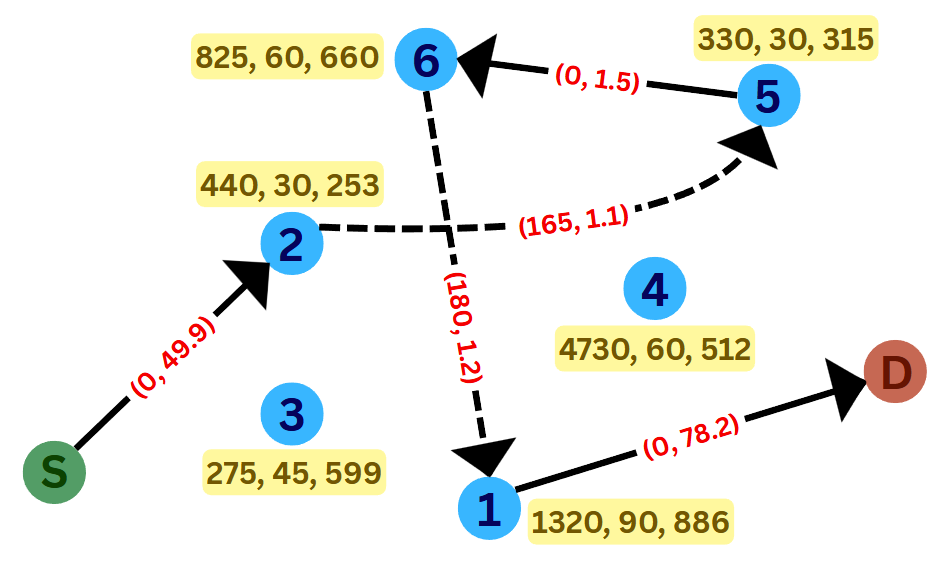
\includegraphics[width=\columnwidth]{plots/updatedExample.png}
	\caption{Example -- \ab{figure needs change}}
	\label{fig:example_graph}
\end{figure}

Consider an example of a toy city that has only 6 POIs.
Table~\ref{tab:example_poi} shows the various time and cost values for
the POIs while Table~\ref{tab:example_walk} and
Table~\ref{tab:example_taxi} shows the travel times among the POIs and
the source and destination marked by $S$ and $D$ respectively for
walking and taxi respectively.

\begin{table}[t]
	\centering
	\resizebox{0.85\columnwidth}{!}
	{
		\begin{tabular}{c l rrr}
			\toprule
			\textbf{ID} & \textbf{Category} & \textbf{Visit Time} & \textbf{Utility} & \textbf{Visit Cost} \\
			\midrule
			%S & Source      & 0  & 0   & 0    \\
			1 & Park        & 90 & 886 & 1320 \\
			2 & Park        & 30 & 253 & 440  \\
			3 & Park        & 45 & 599 & 275  \\
			4 & Museum      & 60 & 512 & 4730 \\
			5 & Museum      & 30 & 315 & 330  \\
			6 & Museum      & 60 & 660 & 825  \\
			%D & Destination & 0  & 0   & 0    \\
			\bottomrule
		\end{tabular}
	}
	\caption{Details of Points of Interests (POIs)}
	\label{tab:example_poi}
\end{table}

\begin{table}[t]
	\centering
	\resizebox{\columnwidth}{!}
	{
		\begin{tabular}{c|cccccccc}
			\toprule
			\textbf{From$\backslash$To} & \textbf{S} & \textbf{1} & \textbf{2} & \textbf{3} & \textbf{4} & \textbf{5} & \textbf{6} & \textbf{D} \\
			\midrule
			\textbf{S} & --    & 28.7  & 49.9  & 55.5  & 68.9  & 126.6 & 117.2 & 102.9 \\
			\textbf{1} & 28.7  & --    & 3.3   & 3.2   & 4.3   & 10.1  & 9.3   & 78.2  \\
			\textbf{2} & 49.9  & 3.3   & --    & 5.7   & 2.7   & 8.0   & 6.9   & 94.3  \\
			\textbf{3} & 55.5  & 3.2   & 5.7   & --    & 5.0   & 9.9   & 9.6   & 47.4  \\
			\textbf{4} & 68.9  & 4.3   & 2.7   & 5.0   & --    & 5.8   & 5.0   & 74.7  \\
			\textbf{5} & 126.6 & 10.1  & 8.0   & 9.9   & 5.8   & --    & 1.5   & 98.5  \\
			\textbf{6} & 117.2 & 9.3   & 6.9   & 9.6   & 5.0   & 1.5   & --    & 102.4 \\
			\textbf{D} & 102.9 & 78.2  & 94.3  & 47.4  & 74.7  & 98.5  & 102.4 & --    \\
			\bottomrule
		\end{tabular}
	}
	\caption{Walking Travel Time Matrix}
	\label{tab:example_walk}
\end{table}

\begin{table}[t]
	\centering
	\resizebox{\columnwidth}{!}
	{
		\begin{tabular}{c|cccccccc}
			\toprule
			\textbf{From$\backslash$To} & \textbf{S} & \textbf{1} & \textbf{2} & \textbf{3} & \textbf{4} & \textbf{5} & \textbf{6} & \textbf{D} \\
			\midrule
			\textbf{S} & --    & 3.8  & 6.7  & 7.4  & 9.2  & 16.9 & 15.6 & 13.7 \\
			\textbf{1} & 3.8   & --   & 0.4  & 0.4  & 0.6  & 1.3  & 1.2  & 10.4 \\
			\textbf{2} & 6.7   & 0.4  & --   & 0.8  & 0.4  & 1.1  & 0.9  & 12.6 \\
			\textbf{3} & 7.4   & 0.4  & 0.8  & --   & 0.7  & 1.3  & 1.3  & 6.3  \\
			\textbf{4} & 9.2   & 0.6  & 0.4  & 0.7  & --   & 0.8  & 0.7  & 10.0 \\
			\textbf{5} & 16.9  & 1.3  & 1.1  & 1.3  & 0.8  & --   & 0.2  & 13.1 \\
			\textbf{6} & 15.6  & 1.2  & 0.9  & 1.3  & 0.7  & 0.2  & --   & 13.7 \\
			\textbf{D} & 13.7  & 10.4 & 12.6 & 6.3  & 10.0 & 13.1 & 13.7 & --   \\
			\bottomrule
		\end{tabular}
	}
	\caption{Taxi Travel Time Matrix}
	\label{tab:example_taxi}
\end{table}

Suppose a traveler has a time and cost budget of 300 and 3500 units respectively.
Additionally, she puts in the contraints that (1)~POIs 1 and 2 must be visited, (2)~POI 2 must be visited before POI 1, and (3)~POI 3, if visited, must be before both POI 2 and POI 5 (if visited).
Further, she must visit at least 2 POIs of the category Park, and will not visit more than 2 POIs of the category Museum.

Respecting all these constraints, the optimal itinerary is $[S, 3, 5,
2, 1, D]$, as shown in Figure~\ref{fig:example_graph}.  Note that the
POIs 4 and 6 were not included.  The total utility obtained from the
itinerary is 1738 units, and the time and cost spent in the itinerary
are, respectively, 3211 ($<$3500) and 256.75 ($<$300) units.

\ignore{

\textbf{Constraints applied:}
\begin{enumerate}[label=\textbf{\arabic*.}]
    \item \textbf{Time budget:} 300 minutes (5 hours)
    \item \textbf{Cost budget:} 3500 units
    \item \textbf{Must-see POIs:} POIs 1 and 2 must be included in the itinerary
    \item \textbf{Ordering constraints:} (Applied if both POIs are included in the itinerary)
    \begin{itemize}
        \item POI 3 must be visited before POI 2
        \item POI 2 must be visited before POI 1
        \item POI 3 must be visited before POI 5
    \end{itemize}
    \item \textbf{Category constraints:}
    \begin{itemize}
        \item At least 2 POIs from the \textit{Park} category
        \item At most 2 POIs from the \textit{Museum} category
    \end{itemize}
    \item \textbf{Modes of travel allowed:} Taxi and walking
\end{enumerate}

\noindent \textbf{Itinerary suggested in Binary Version:}
Start from S, spend exact amount of visiting time on POIs 1,2 and 3 and gain complete utility from them, reach D.
\begin{itemize}
    \item \textbf{Utility Score:} 1738
    \item \textbf{Total trip cost:} 3211 units
    \item \textbf{Total time taken:} 256.75 minutes
\end{itemize}

\noindent \textbf{Itinerary suggested in Fractional Version}\\
\textbf{Variant of utility calculation: Continuous Linear Function}
Start from S, arrive on 3, visit it completely and gain full utility, arrive on 5, visit it completely and gain full utility, arrive on 2, spend 28.14 minutes here instead of 30 minutes, gain proportional utility, then arrive on 1, spend complete visiting time and gain full utility, then reach destination.
\begin{itemize}
    \item \textbf{Utility Score:} 2037.31
    \item \textbf{Total trip cost:} 3475.25 units
    \item \textbf{Total time taken:} 300 minutes
\end{itemize}

\noindent \textbf{Variant of utility calculation: Slabs}
Same itinerary as CLF variant except on POI 2, the utility granted to tourist was $28.14/30$
which is $0.938$ times the complete utility i.e. $237.314$, Here in slabs variant, spending $93.8\%$ utility grants $90\%$ of complete utility according to Slab 5, and tourist will gain the same utility on POI 2 if he spends $27$ minutes here, hence utility granted is $227.7$ and time spent is $27$ minutes instead of $28.14$ minutes.
\begin{itemize}
    \item \textbf{Utility Score:} 2027.7
    \item \textbf{Total trip cost:} 3475.25 units
    \item \textbf{Total time taken:} 298.86 minutes
\end{itemize}

\noindent \textbf{Insights}
\begin{itemize}
    \item Fractional Version gains ~$17\%$ more utility than Binary Version.
    \item More effecient Time and Cost budget utilization can be observed in the Fractional version.
    \item The Slabs variant gives approximately similar utility as CLF variant with slight changes due to the modelling of slabs.
\end{itemize}

}

